\chapter{Implementación}

	\section{¿Qué es una FPAA?}
	Una FPAA  por sus siglas en inglés (Field Programmable Analog Arrays) es un dispositivo analógico equivalente a las FPGA (Field Programmable Garte Arrays). A diferencia de las FPGA que contienen una gran cantidad de módulos y conexiones que permiten configuraciones arbitrarias de lógica combinacional y secuencial, los FPAA generalmente contienen una pequeña cantidad de CABs (Configurable Analog Blocks). Los FPAA dirigidos al diseño analógico estándar generalmente presentan un CAB que contiene un amplificador operacional, un arreglo de capacitores programables, y ya sea un arreglo de resistencias programables para circuitos en tiempo continuo o switches configurables para circuitos de capacitores conmutados.
	Se trabajó con la tarjeta Anadigm QuadApex Develovment Boarsd v2.0 de la empresa Anadigm, la cual contiene 4 FPAAs AN231E04 que pueden conectarse en cadena y es programada mediante el software AnadigmDesigner2 (AD2). 
	
	\section{AnadigmDesigner2}
	
	AD2 trabaja con módulos llamados CAMs (Configurable Analog Modules), estos aportan flexibilidad y sencillez en el proceso diseño debido a que son bloques que hacen desde funciones sencillas como inversores o comparadores hasta diseños completos como filtros y multiplicadores, los CAMs se pueden interconectarse fácilmente unos con otros y únicamente necesitan pequeñas configuraciones para su correcto funcionamiento. Los CAMs más utilizados en el diseño de osciladores caoticos son los mostrados en la Tabla \ref{tab:CAMs_AD2}
	

\begin{table}[!ht]
  \centering
  \caption{CAMs básicos de AD2}
  \label{tab:CAMs_AD2}
  \begin{tabular}{>{\centering\arraybackslash}m{3cm} >{\centering\arraybackslash}m{5cm} >{\centering\arraybackslash}m{5cm}}
    \hline
    \textbf{Nombre} & \textbf{Función de transferencia} & \textbf{Descripción}\\ 
    \hline
    {\scriptsize \textbf{GainInv}}
    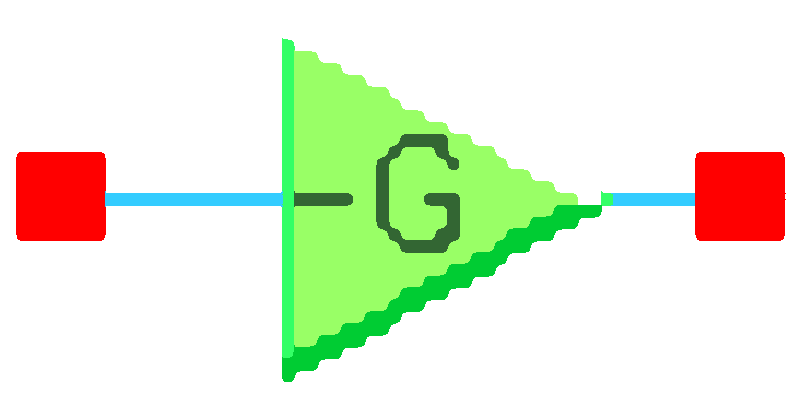
\includegraphics[width=2.2cm]{T7_Inversor.eps}
    &
      $\frac{V_{\mathrm{out}} (s)}{V_{\mathrm{in}}(s)} = - G$
    & 
      \begin{itemize}[leftmargin=0cm,noitemsep]
      \begin{scriptsize}
		\item[] Ganancia inversora.
		\item[] Gain: 0.01 - 100.0 V/V
      \end{scriptsize}
      \end{itemize}
    \\ %-------------------------------------------------------
    {\scriptsize \textbf{Integrator}}
    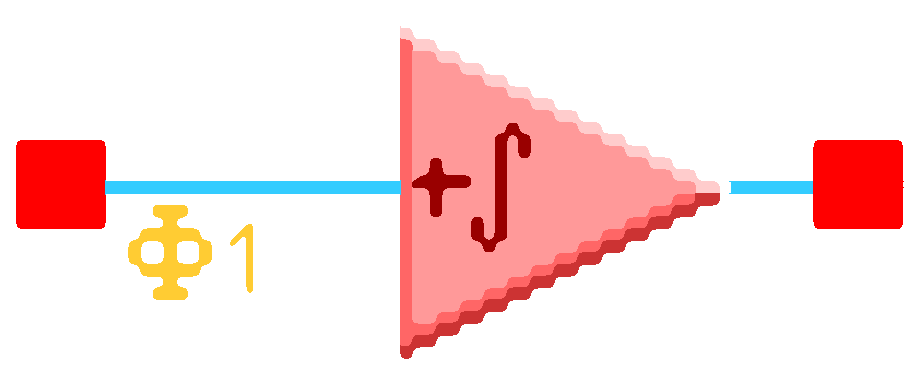
\includegraphics[width=2.5cm]{T1_Integrador.eps}
    &
      $ \frac{V_{\mathrm{out}} (s)}{V_{\mathrm{in}}(s)} = \frac{\pm K}{s}$
    & 
      \begin{itemize}[leftmargin=0cm,noitemsep]
      \begin{scriptsize}
		\item[] Integrador con una constante de integración programable. La salida puede ser inversora o no inversora.
      \end{scriptsize}
      \end{itemize}
    \\ %-------------------------------------------------------
    {\scriptsize \textbf{Voltage}} \linebreak
    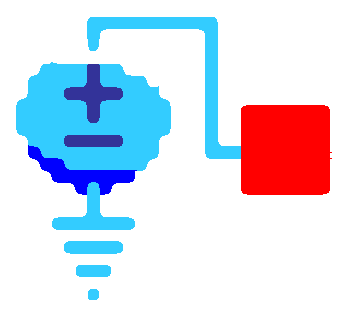
\includegraphics[width=1cm]{T6_DC_voltage.eps}
    &
      $V_{\mathrm{out}} = \pm 2$
    & 
      \begin{itemize}[leftmargin=0cm,noitemsep]
      \begin{scriptsize}
		\item[] Referencia de voltaje de $\pm$ 2 V.
      \end{scriptsize}
      \end{itemize}
    \\ %-------------------------------------------------------
    {\scriptsize \textbf{TransferFunction}} \linebreak
    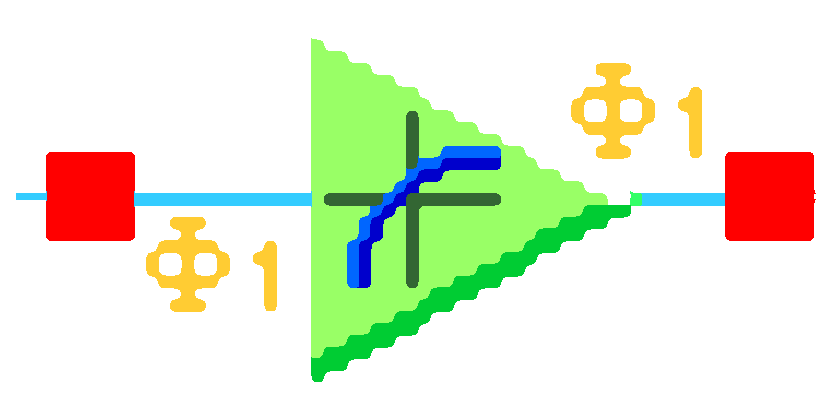
\includegraphics[width=2.5cm]{T3_Transferfunction.eps}
    &
    & 
      \begin{itemize}[leftmargin=0cm,noitemsep]
      \begin{scriptsize}
		\item[] \textbf{Lookup Table}: función de transferencia especificada por el usuario de 256 de pasos de cuantificación.  
      \end{scriptsize}
      \end{itemize}
    \\ %-------------------------------------------------------
    {\scriptsize \textbf{Multiplier}} \linebreak
    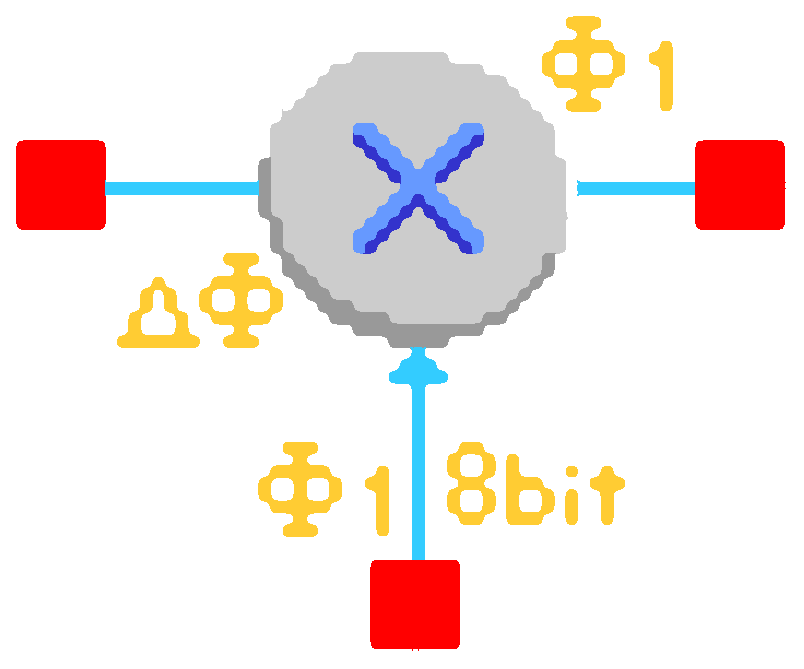
\includegraphics[width=2.5cm]{T2_Multiplicador.eps}
    &
      $V_{\mathrm{out}} = M \cdot V_{x} \cdot V_{y}$
    & 
      \begin{itemize}[leftmargin=0cm,noitemsep]
      \begin{scriptsize}
		\item[] $V_{x}$ es la entrada de voltaje izquierda.
		\item[] $V_{y}$ es la entrada de voltaje inferior cuantificado de 8 bits.
		\vspace{-0.15cm}
		\item[] $M$ factor de multiplicación.
      \end{scriptsize}
      \end{itemize}
    \\ %-------------------------------------------------------
    {\scriptsize \textbf{SumDiff}} \linebreak
    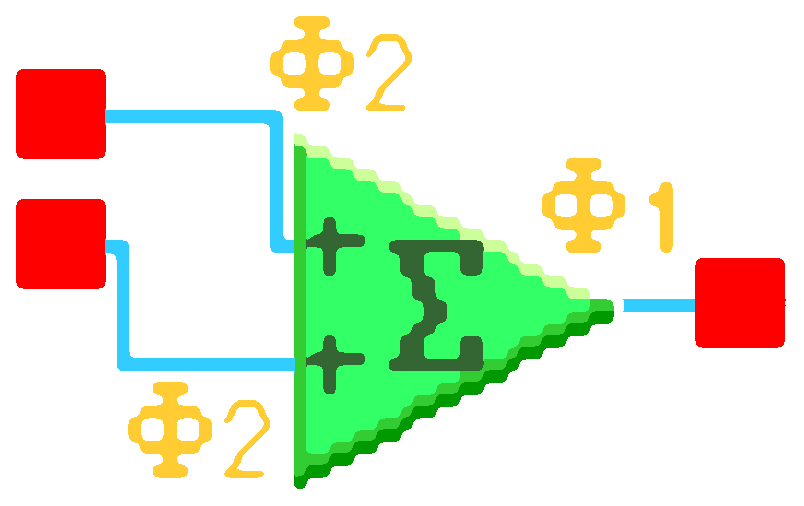
\includegraphics[width=2.5cm]{T8_Sumador.eps}
    &
      \begin{footnotesize}
      	$V_{\mathrm{out}} = \pm G_{1} V_{\mathrm{in1}} \pm G_{2} V_{\mathrm{in2}} \pm G_{3} V_{\mathrm{in3}} \pm G_{4} V_{\mathrm{in4}}$
      \end{footnotesize}
    & 
      \begin{itemize}[leftmargin=0cm,noitemsep]
      \begin{scriptsize}
		\item[] Las entradas pueden ser inversoras o no inversoras.
		\item[]	Cada entrada tiene una ganancia programable.
		\vspace{-0.15cm}
		\item[] Configurable desde 2 hasta 4 entradas. 
      \end{scriptsize}
      \end{itemize}
    \\ %-------------------------------------------------------
    {\scriptsize \textbf{FilterBilinear}} \linebreak
    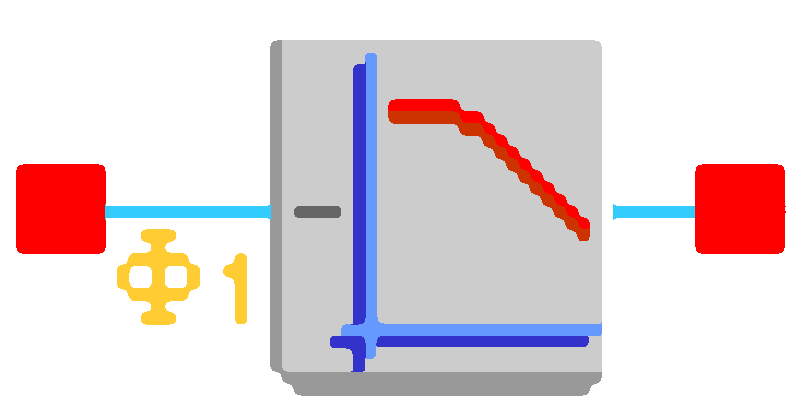
\includegraphics[width=2.5cm]{T9_FilterBilinear.eps}
    &
      \begin{scriptsize}
		 \textbf{Low Pass Bilinear Filter} \linebreak
      	 $\frac{V_{\mathrm{out}}(s)}{V_{\mathrm{in}}(s)} = \pm \frac{2 \pi f_{0} G}{s + 2 \pi f_{0}}$ \linebreak
      	 \textbf{High Pass Bilinear Filter} \linebreak
      	 $\frac{V_{\mathrm{out}}(s)}{V_{\mathrm{in}}(s)} = - \frac{Gs}{s + 2 \pi f_{0}}$ \linebreak
      	 $\vdots$
      \end{scriptsize}
    & 
      \begin{itemize}[leftmargin=0cm,noitemsep]
      \begin{scriptsize}
		\item[] Puede ser configurado como pasa
      \end{scriptsize}
      \end{itemize}
    \\ %-------------------------------------------------------
    {\scriptsize \textbf{FilterBiquad}} \linebreak
    \includegraphics[width=2.5cm]{T10_FilterBiquad.eps}
    &
      \begin{scriptsize}
		 \textbf{Low Pass Biquadratic Filter} \linebreak
      	 $\frac{V_{\mathrm{out}}(s)}{V_{\mathrm{in}}(s)} = \frac{\pm 4 \pi^{2} f_{0}^{2} G}{s^{2} + \frac{2 \pi f_{0}}{Q}s + 4 \pi^{2} f_{0}^{2}}$ \linebreak
      	 \textbf{High Pass Biquadratic Filter} \linebreak
      	 $\frac{V_{\mathrm{out}}(s)}{V_{\mathrm{in}}(s)} = \frac{-G s^{2}}{s^{2} + \frac{2 \pi f_{0}}{Q} s + 4 \pi^{2} f_{0}^{2}}$ \linebreak
      	 $\vdots$
      \end{scriptsize}
    & 
      \begin{itemize}[leftmargin=0cm,noitemsep]
      \begin{scriptsize}
		\item[] \textbf{Integration Const}: 0.00250 
      \end{scriptsize}
      \end{itemize}
    \\ %-------------------------------------------------------
    \hline
  \end{tabular}
\end{table}
